\subsection{Treatments for ansatzes}
\todo{add method 2 and 3}
We apply the methods in Section \ref{Research Design section} to the ansatzes.

\subsubsection{Method \#0: Unrestricted}
As discussed in the Section \ref{Research Design section}, the goal of this configuration is to produce a general multilayered perceptron network without any restriction.
The ansatzes will have unrestricted growth of circuit depth with a global cost function.
The initial parameters of this ansatz are randomised.
We implement the default ansatz to have the number of qubits and repetition increased iteratively.

\subsubsection{Method \#1: Local Cost Function and Shallow Depth Implementation}
We implemented the \textit{Global Cost Function} as the measurement output for all qubits, while the \textit{Local Cost Function} is the measurement for the first two qubits.
Section \ref{Shallow Circuits, Local Cost Function section} and figure \ref{cost functions} previously explained the differences between the two cost functions.
The shallow ansatz is the same as the default.
However, the repetition number is kept as a constant number.

\subsubsection{Method \#2: Layerwise Learning}
The ansatses will have unrestricted growth of circuit depth, and a measurement gate for each qubit at the end as the global cost function.
While the construction process is similar to that of the method \#0, we follow the \emph{Layerwise learning} as described in Section \ref{Sec: Layerwise Learning} to obtain the optimal initial parameters.

\subsubsection{Method \#3: Identity Blocks}
For this method, we create a custom ansatz as an identity block.
As discussed in Section \ref{Sec: Identity blocks}, one identity block has two part, the first part can have its parameter randomised, while the second part invert the first part.
Figure \ref{Fig: Identity Ansatz Sample} demonstrate an identity block with two qubits.
For the first part of the identity block, we use the Real amplitudes with one repetition layer plus one rotation layer.
The gates of this part has their parameters randomised.
The second part of the identity block simply reverse the sequence of rotation layers and entanglement layers.
The gates of this part has their parameters chosen as invert of the first layer.
\begin{figure}
    \centering
    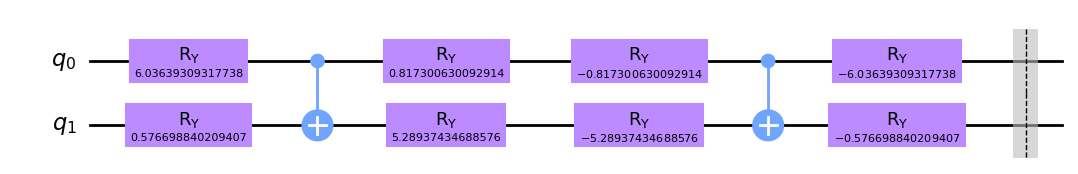
\includegraphics[width=\textwidth]{Artefact/Appendices/ansatz-identity.png}
    \caption{An Identity Block of two qubits, the first part has four random parameters, the second part is an invert of the firt part.}
    \label{Fig: Identity Ansatz Sample}
\end{figure}
